\label{chap:results}

In this chapter we will cover the results obtained with this gateway platform
and other possible applications.

\begin{figure}[ht] \centering
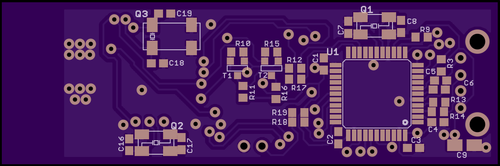
\includegraphics[width=0.3\textwidth]{img/dongleb.png} \caption{Bottom side of
SparrowDongle PCB} \end{figure}


\begin{figure}[ht] \centering
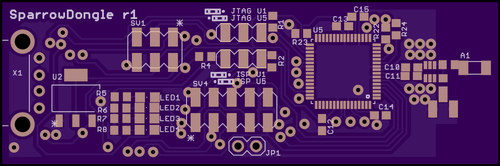
\includegraphics[width=0.3\textwidth]{img/donglef.png} \caption{Top side of
SparrowDongle PCB} \end{figure}

\subsection{Performance}

Throughput testing was done with back-to-back packets sent at 250kbps over
2.4GHz with one sending node in acceptable range, with no losses. This is due
to the double-buffering used in receiving packets from the wireless network.
As soon as one packet ends, a signal is sent to the radio controller unit with
a small delay of 9$\mu S$. Even if a new packet starts in that small interval,
receipt of the new packet goes unhindered as the first bytes of the old packet
have already been transfered to a different memory location from which they
will be sent to the USB controller unit via the serial connection.

\subsection{Software configurations}

A great advantage of using a dedicated USB Controller Unit for the gateway is
that it can be programmed as one of several USB Communication Classes. The USB
Controller Unit is not limited in implementing any of these classes since most
of the computing power at its disposal is reserved for USB.  SparrowDongle can
appear as different USB devices:

\begin{itemize}

\item \textit{Virtual Serial Port}: Communication with the wireless island
around the gateway can be made via a serial link, incoming packets will appear
on the receive end of this port and packets will be sent on the transmit end.
In typical Unix fashion, our implementation sends packet in ASCII for ease of
use and debugging. They are converted to binary form on the Radio Controller
Unit of the gateway

\item \textit{Ethernet Emulation}: In this fashion, packets are received on the
gateway and then encapsulated in an Ethernet packet sent over the USB link
(Ethernet is emulated between the USB device and USB host)

\item \textit{Network card}: SparrowDongle behaves as a wireless network card,
the operating system will register a network interface for the gateway and
addresses assigned to this interface will change the gateway's address in the
wireless medium (as opposed to changing the address for the emulated Ethernet)

\item \textit{Mass Storage}: SparrowDongle can offer a virtual filesystem
interface for innovative data acquisition from the wireless sensor network. In
accordance with the Unix philosophy of "everything is a file", the virtual
filesystem offered by the USB stick could have a file for each wireless node
where it stores recent data (as much as the gateway can store in its volatile
memory, 1-2 records per node). The software implementation for this interface
is under development.

 \end{itemize}

\subsection{Applications}


The versatility of the SparrowDongle gateway platform allows it to be deployed
in a wide range of applications, whether the gateway has to be connected to a
PC or a small embedded device, whether it has to implement a virtual serial
connection or to emulate an ethernet link.

For instance, these are the application in which SparrowDongle is currently
deployed:

 \begin{itemize} 

\item Connected to a Windows PC, feeding wireless sensor data into a service
framework for building control, in the FCINT project. \cite{fcint}

\item Connected to an Embedded Linux board, such as the small RaspberryPi, for
plug-and-play monitoring of a wireless sensor island.

\item Connected to a Parrot Drone \cite{parrot2012drone}, for remote monitoring
using a mobile gateway. 

\end{itemize}

